\section{Partitioning Schemes}
\label{SECTION:PARTITIONING_SCHEMES}
\subsection{Rationale}
Before diving into the results for this experiment, we now explain two partition strategies to take into consideration before designing our first experiment and our second algorithm modification in order to understand the modifications made to IQS.

\subsection{Partition schemes}
As explained before in~\ref{SEC:INCREMENTAL_SORTING}, partition algorithms play a fundamental role on sorting algorithms like QuickSort. But partition algorithms can use different schemes in order to partition the array into two sections, depending on which properties of the process we want to optimise.

\subsection{Lomuto's partition scheme}

The most noticeable feature of this algorithm is that it uses the last element as the pivot for partitioning the array, which makes suitable for shuffled sequences but when the sequence follows some of the first disorder metrics seen in~\ref{SEC:MEASURING_DISORDER} it tends to bias the performance of this partition scheme.

This algorithm is commonly referenced as the easiest way to partition an array, given it is low complexity.
o
\begin{algorithm}
\caption{Lomuto Partition}\label{ALG:LOMUTO_PARTITION}
\begin{algorithmic}[1]
    \Procedure{$lomuto$}{$A, p, r$}
    \State $x \gets A_r$
    \State $i \gets p-1$
    \For{$j \in [p, r - 1]$}
    \If{$A_j \leq x$}
        \State $i \gets i + i$
        \State $swap(A_i, A_j)$
    \EndIf
    \EndFor
    \State $swap(A_{i+1}, A_r)$
    \State \Return $i + 1$
    \EndProcedure
\end{algorithmic}
\end{algorithm}

\subsection{Hoare's partition scheme}
Hoare's partition scheme takes another approach at partitioning elements by using two indices which converge into the position of the pivot chosen at the beginning. When it comes to sort a set of elements it works faster than Lomuto's implementation and it's more stable. and given that the pivot can be chosen randomly, the introduction of randomness helps to ease biased pivot selections.

\begin{algorithm}
\caption{Hoare's Partition}\label{ALG:HOARE_PARTITION}
\begin{algorithmic}[1]
    \Procedure{$hoare$}{$A, p, r$}
    \State $x \gets A_p$
    \State $i \gets p-1$
    \State $j \gets r+1$
    \While{$true$}
        \Do 
            \State $j \gets j - 1$
        \doWhile{$A_j \leq x$}

        \Do 
            \State $i \gets i + 1$
        \doWhile{$A_j \geq x$}

        \If{$i < j$}
            \State $swap(A_i, A_j)$
        \Else
            \State \Return $j$
        \EndIf
    \EndWhile
    \EndProcedure
\end{algorithmic}
\end{algorithm}

\subsection{Dutch flag problem}
\label{SUBSEC:DUTCH_FLAG_PROBLEM}
Both of the aforementioned algorithms were designed to operate on sets, but when it comes to sequences, to use such partition methods fails dramatically. As it treats repeated elements as unique elements, in worst case, the pivot is positioned into its corresponding place but it does not guarantee that there are no repetitions of the same element on any portion of the original sequence.

\subsection{Problem definition and solution}
\label{SUBSECITON:PARTITIONING_PROBLEM}
Let us take as example the partitioning problem of the following two sequences:

$$ S_1={1,2,3,4,5,6,7,8,9} $$
and
$$S_2={1,2,5,5,5,5,5,8,9}$$

It is clear that if we chose $p$ equal to $5$, the element in the fifth position of $S_1$ is the pivot on its correct place. But it is not the case for $S_2$ as we can get a pivot from the third up to the seventh position on the sequence. In this case, as all the positions are valid pivots as they are following the definition of partitioning. There is no safety guarantee that the resulting pivot  partitions the array in half in order to ensure a $log_2$ decay on the problem space. Situation worsens if all the elements are repeated, as it defeats the purpose of partitioning the sequence~\cite{7416566}.

This problem is also known as the Dutch Flag problem~\cite{10.5555/550359}, which for given a sequence it partition in-place the elements lower than the pivot value, the elements equal to the pivot value and the elements greater than the pivot value and it returns the indices of the beginning and the end of the middle portion.

\begin{algorithm}
\caption{Three-way Partition}\label{ALG:DUTCH_FLAG_PARTITION}
\begin{algorithmic}[1]
    \Procedure{$threewaypartition$}{$A, p$}
    \State $k \gets \norm{A}$
    \State $i \gets 0$
    \State $j \gets 0$
    \While{$j < k$}
        \If{$A_j < p$}
            \State $swap(A_i, A_j)$
            \State $i \gets i+1$
            \State $j \gets j+1$
        \ElsIf{$A_j > p$}
            \State $k \gets k-1$
            \State $swap(A_i, A_k)$
        \Else
            \State $j \gets j+1$
        \EndIf
    \EndWhile
    % \State \Return $i,J,k$
    \EndProcedure
\end{algorithmic}
\end{algorithm}

\subsection{Integration into IQS as base implementation}

It makes no sense to check our base partition implementation against repeated elements, as its behaviour is undefined. But we can do the opposite, to test our dutch-flag implementation in order to check if the time bounds are equivalent to each other. In this regard, we are not to make asumptions that the following test apply for all implementations available of partition-based sorting algorithms.

\begin{figure}[!ht]
    \centering
    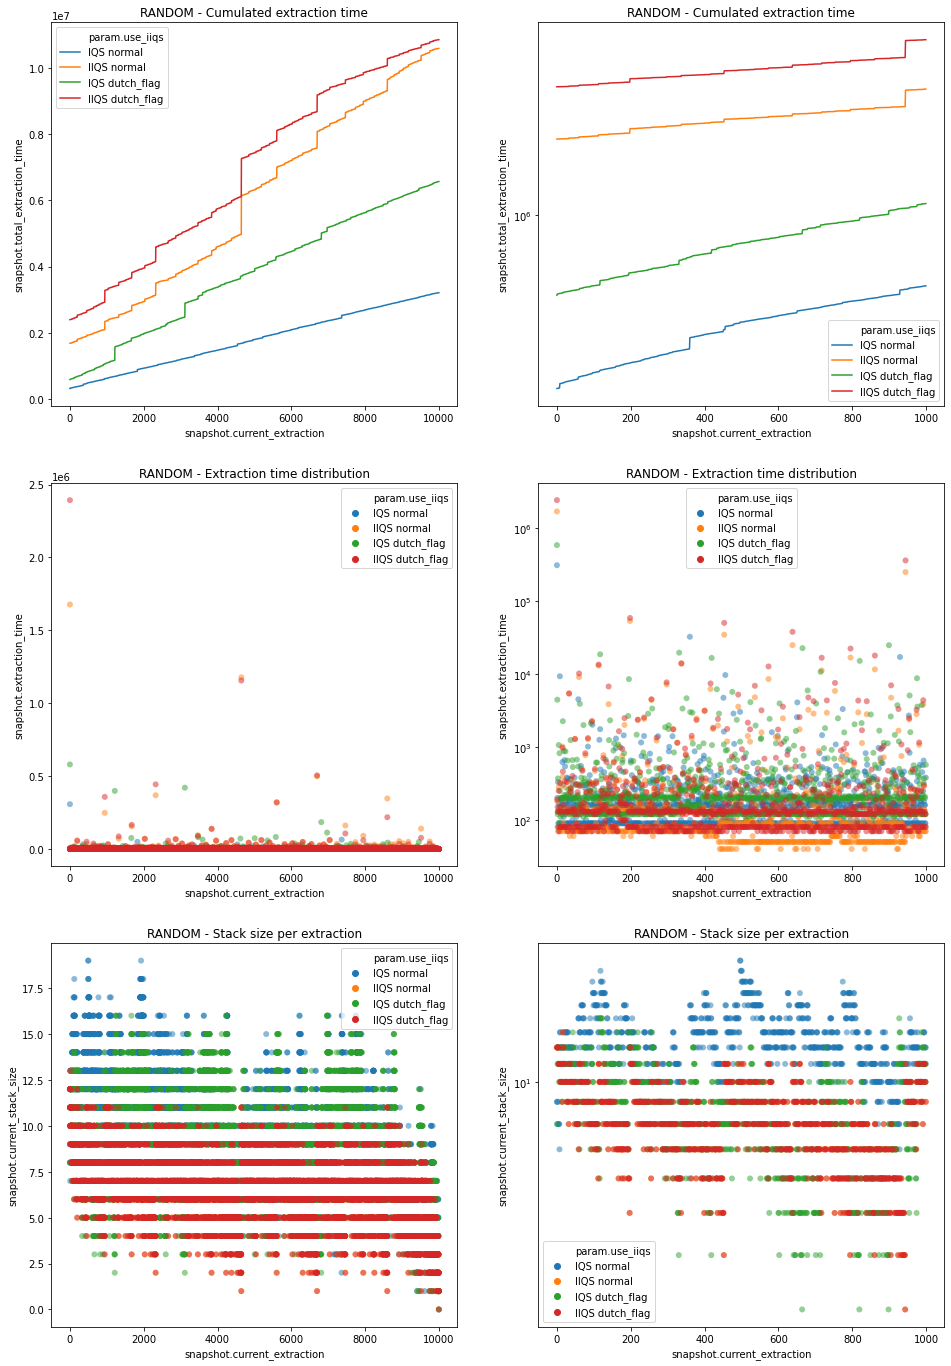
\includegraphics[width=0.8\textwidth]{./fragments/04_experimental_execution/images/02_basebenchmark_01_base_benchmark.png}
    \caption{Performance comparison for different partition implementations on IQS and IIQS using a shuffled input sequence. First column represents all extractions using a linear scale. Second column depicts a logarithmic scale and shows the first $1\times10^3$ extractions.}
    \label{FIG:PARTITION_SCHEME_01_SHUFFLED}
\end{figure}

As depicted in Figure \ref{FIG:PARTITION_SCHEME_01_SHUFFLED}, there is no noticeable change in terms of complexity for both implementations of the partitioning algorithm when dealing with shuffled sequences. As such, it does result interesting how for IIQS both implementations of partition break up the array at the same index, which confirms that both implementations perform the same operations in the same order. On the other hand, it does look that for IQS there is a scalar overhead which seems to be reduced over time. 

\begin{figure}[!ht]
    \centering
    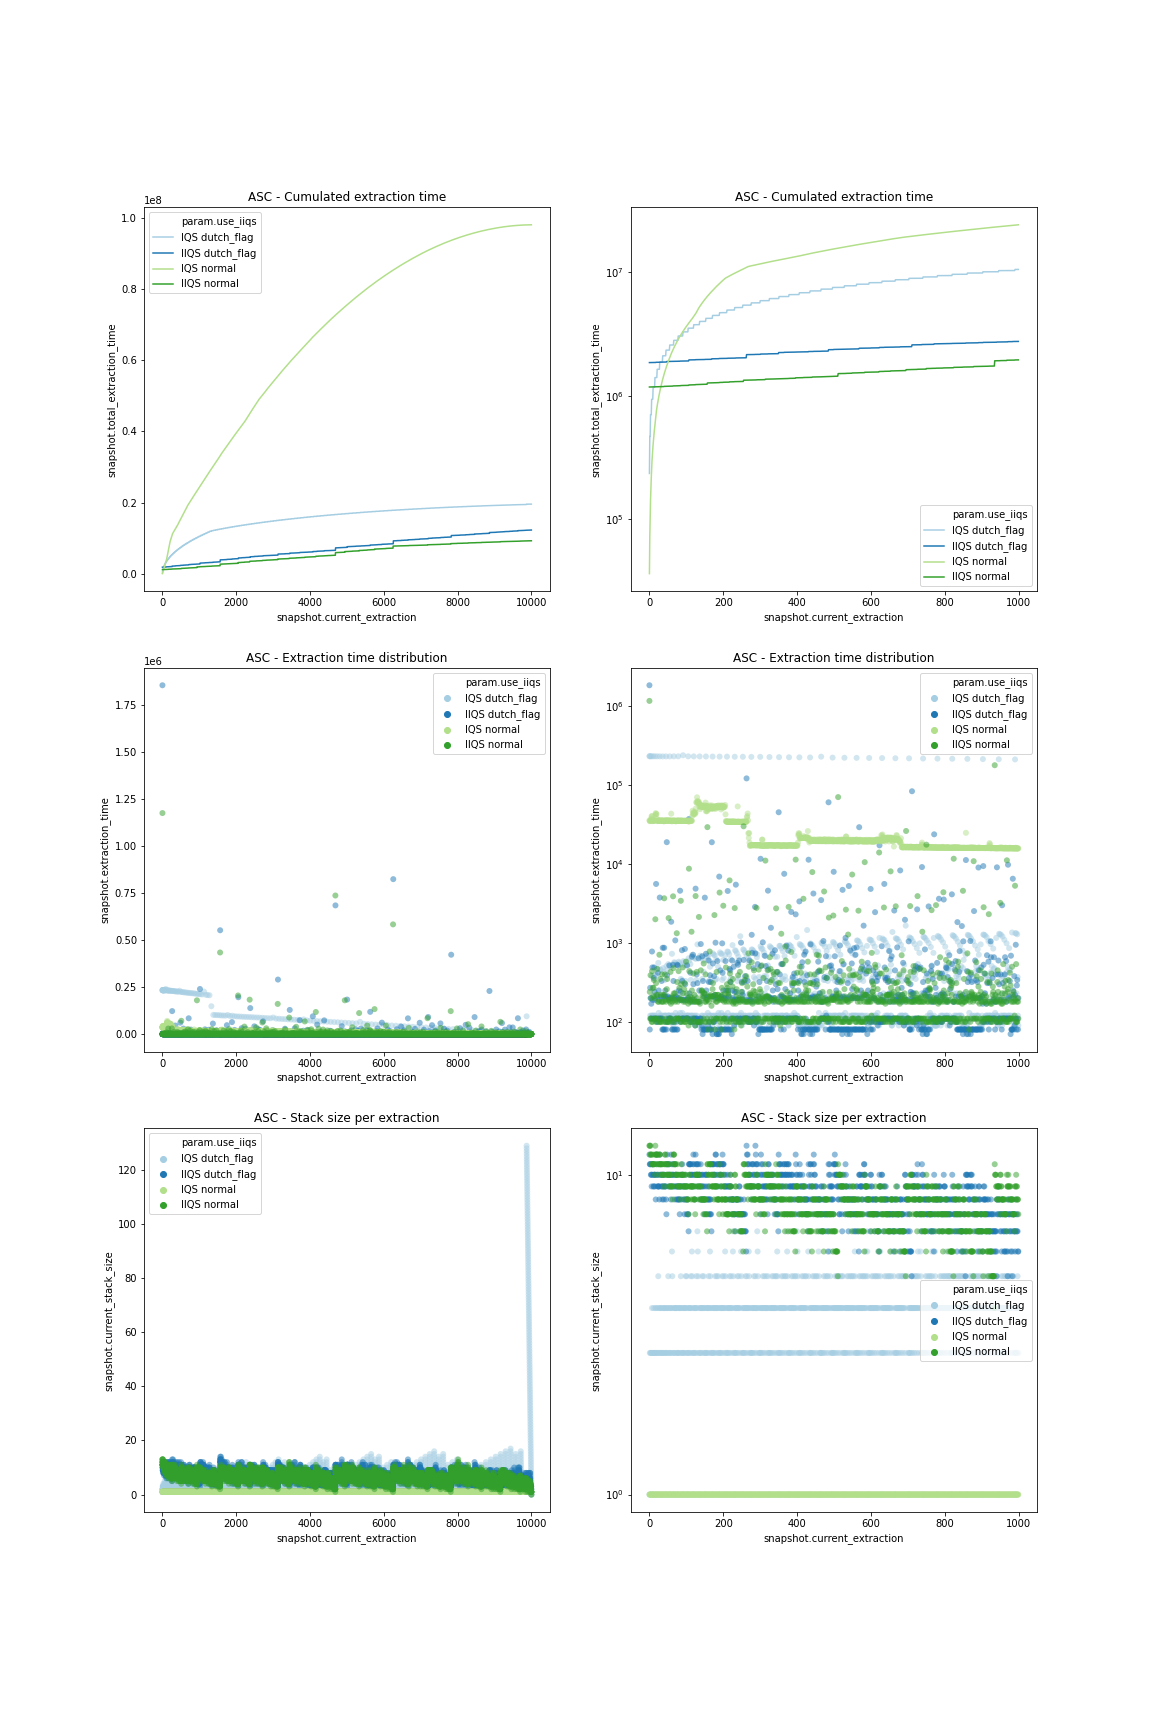
\includegraphics[width=0.8\textwidth]{./fragments/04_experimental_execution/images/02_benchmark_02_sort_a_case.png}
    \caption{Performance comparison for different partition implementations on IQS and IIQS using a ascending input sequence. First column represents all extractions using a linear scale. Second column depicts a logarithmic scale and shows the first $1\times10^3$ extractions.}
    \label{FIG:PARTITION_SCHEME_01_ASCENDING}
\end{figure}

\begin{figure}[!ht]
    \centering
    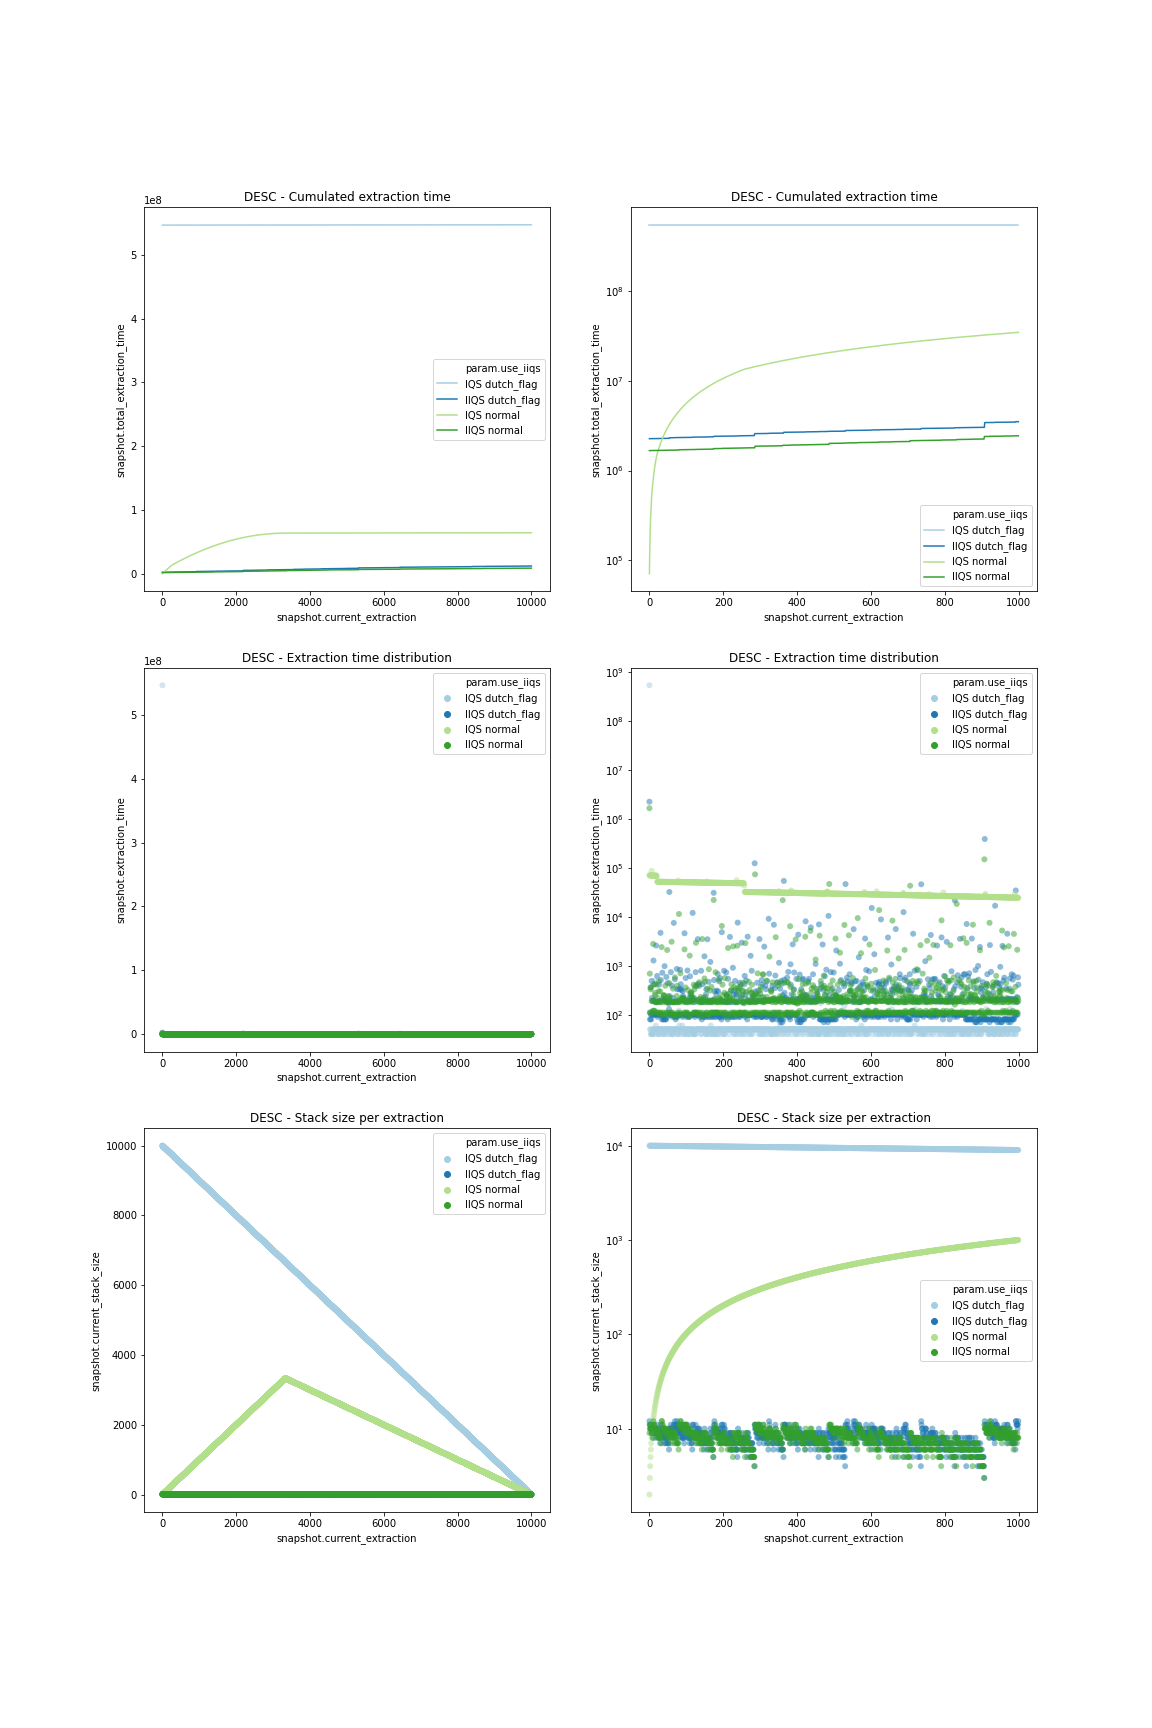
\includegraphics[width=0.8\textwidth]{./fragments/04_experimental_execution/images/02_basebenchmark_03_sort_d_case.png}
    \caption{Performance comparison for different partition implementations on IQS and IIQS using a descending input sequence. First column represents all extractions using a linear scale. Second column depicts a logarithmic scale and shows the first $1\times10^3$ extractions.}
    \label{FIG:PARTITION_SCHEME_01_DESCENDING}
\end{figure}

Figure \ref{FIG:PARTITION_SCHEME_01_ASCENDING} and Figure \ref{FIG:PARTITION_SCHEME_01_DESCENDING} confirms our hypothesis in Section~\ref{SUBSECTION:BASE_BENCHMARK__AVERAGE_WORST} about the different behaviour of IQS and IIQS when dealing with repeating sequences and how the stack is consumed, validating our base benchmark results.

Apart from those behaviour deviations, there no noticeable difference between running time of our implementations for three-way partitioning and standard partitioning algorithms in terms of complexity. As such, from now on we use \textit{three-way-partition} as our default implementation for the partitioning stage. This allows us to contrast results between IQS and IIQS with such modifications using both repeated and non repeated elements as dataset inputs under the same partitioning conditions.

\FloatBarrier